\begin{exercisePage}[Kompakte Konvergenz, Integralberechnung, Nullhomologie \& --homotopie]
	
	\begin{task}
		Sei $\Omega \subseteq \Rn$ offen, $(f_n)$ eine Folge von stetigen Funktionen $\abb{f_n}{\Omega}{\CC}$ und $\abb{f}{\Omega}{\CC}$. Zeigen Sie die Äquivalenz folgender Aussagen:
		\begin{enumerate}[label=(\roman*), leftmargin=*, nolistsep]
			\item $(f_n)$ ist kompakt konvergent gegen $f$, d.h. gleichmäßig konvergent auf kompakten Teilmengen von $\Omega$: Für alle $K \subseteq \Omega$ kompakt mit $K \neq \emptyset$ gilt
			\begin{equation*}
				\sup\menge{\abs{f(\zeta) - f_n(\zeta)} : \zeta \in K} \to 0 \qquad (n \to \infty)
			\end{equation*}
			\item $(f_n)$ ist lokal gleichmäßig konvergent gegen $f$, d.h. für alle $z \in \Omega$ gibt es eine Umgebung $U \subseteq \Omega$ von $z$, sodass
			\begin{equation*}
				\sup\menge{\abs{f(\zeta) - f_n(\zeta)} : \zeta \in U} \to 0 \qquad (n \to \infty)
			\end{equation*}
		\end{enumerate}
	\end{task}
	
	\begin{equivalence}
		\hinrichtung Sei $f_n \to f$ kompakt und $z \in \Omega$. Da $\Omega$ offen ist, existiert eine Umgebung $B_\epsilon(z) \subseteq \Omega$ mit $\quer{B_\epsilon(z)} \subseteq \Omega$. Da $\quer{B_\epsilon(z)}$ beschränkt und abgeschlossen ist, ist $\quer{B_\epsilon(z)}$ kompakt. Nach Voraussetzung konvergiert also $f_n \to f$ gleichmäßig auf $\quer{B_\epsilon(z)}$, d.h. $\sup\menge{\abs{f(\zeta) - f_n(\zeta)} : \zeta \in \quer{B_\epsilon(z)}} \to 0$. Somit ist auch $\sup\menge{\abs{f(\zeta) - f_n(\zeta)} : \zeta \in B_\epsilon(z)} \to 0$ für alle $z \in \Omega$ und daher $f_n \to f$ lokal gleichmäßig.
		\rueckrichtung Sei $f_n \to f$ lokal gleichmäßig, d.h. für jedes $z \in \Omega$ existiert ein $\epsilon > 0$, sodass $B_\epsilon(z) \subseteq \Omega$ und $\sup\menge{\abs{f(\zeta) - f_n(\zeta)} : \zeta \in B_\epsilon(z)} \to 0$. Sei nun $K \subseteq \Omega$ eine beliebige kompakte Menge und $\folge{B_\epsilon(z)}{z \in K}$ eine offene Überdeckung von $K$ mit $f_n \to f$ gleichmäßig auf jeder Umgebung $B_\epsilon(z)$ ($z \in K$). Aufgrund der Kompaktheit von $K$ existiert eine endliche Teilüberdeckung $\menge{B_{\epsilon_i}(z_i)}_{i=1}^n$. Sei $\epsilon > 0$. Aufgrund der gleichmäßigen Konvergenz existiert dann für $1 \le i \le n$ ein $N_i$, sodass $\sup\menge{\abs{f(\zeta) - f_n(\zeta)} : \zeta \in B_\epsilon(z)} < \epsilon$ für alle $n > N_i$. Setze nun $N \defeq \max\menge{N_i : 1 \le i \le n}$ und $B \defeq \bigcup_{i=1}^n B_{\epsilon_i}(z_i)$. Dann ist $\sup\menge{\abs{f(\zeta) - f_n(\zeta)} : \zeta \in B} < \epsilon$ für alle $n > N$, d.h. $\sup\menge{\abs{f(\zeta) - f_n(\zeta)} : \zeta \in B} \to 0$ für $n \to \infty$. Somit konvergiert $f_n \to f$ gleichmäßig auf $B$, also auch auf dem beliebigen Kompaktum $K$ und daher ist $f_n$ kompakt konvergent gegen $f$.
	\end{equivalence}

	
	\begin{task}
		Sei $\abb{f}{\CC}{\CC}$ stetig und die Einschränkung von $f$ auf $\menge{z \in \CC : \Re(z) \neq 0}$ sei holomorph. Zeigen Sie, dass
		\begin{equation*}
			\int_{\triangle(a,b,c)} f(z) \dz = 0
		\end{equation*} 
		für alle $a,b,c \in \CC$. Mit dem Satz von Morera ist dann $f$ holomorph. 
		
		Hinweis: Zeigen Sie zuerst, dass $\int_\gamma f(z) \dz = 0$ für jeden geschlossenen Weg $\abb{\gamma}{[a,b]}{\menge{z \in \CC : \Re(z) \ge 0}}$.
	\end{task}

	\pagebreak

	Sei $\CC^+ \defeq \menge{z \in \CC : \Re(z) > 0}$ und $\quer{\CC^+} \defeq \menge{z \in \CC : \Re(z) \ge 0}$. Wir wollen zeigen, dass $\CC^+$ sternförmig ist, d.h. es existiert ein $z_0 \in \CC^+$, sodass $\im(\sigma_{z_0,z}) \subseteq \CC^+$ für alle $z \in \CC^+$. Wähle $z_0 = 1$. Dann ist für jeden Punkt $z$ der rechten Halbebene auch die Verbindungsstrecke $\im(\sigma_{z_0, z})$ in der rechter Halbebene. Für einen stückweise stetig differenzierbaren und geschlossenen Weg $\abb{\gamma}{[a,b]}{\quer{\CC^+}}$ betrachten wir den Weg $\gamma + \epsilon$ für ein $\epsilon > 0$. Dieser liegt dann vollständig in $\CC^+$. Dort ist $f$ holomorph und nach dem Cauchyschen Integralsatz gilt dann $\int_{\gamma + \epsilon} f(z) \dz = 0$. 
	
	Sei nun $\epsilon_n \to 0$. Definiere $f_n(\gamma(t)) \defeq f(\gamma(t) + \epsilon_n)$. Dann gilt wegen der Stetigkeit von $f$, dass $f_n(\gamma(t)) \to f(\gamma(t))$ für $n \to \infty$, d.h. $f(\gamma(t) + \epsilon) \to f(\gamma(t))$ für $\epsilon \to 0$.
	$\gamma$ ist stückweise stetig differenzierbar, d.h. wir betrachten eine Unterteilung $a = t_0 < t_1 < \dots < t_n = b$ und notieren $\mathcal{I}_i \defeq [t_i, t_{i+1}]$ für alle $i \in \menge{0, \dots, n-1}$. Aufgrund der Stetigkeit von $f$ und der Stetigkeit von $\gamma$ auf $\mathcal{I}_i$ ist $f \circ \gamma$ stetig auf kompaktem $\mathcal{I}_i$ für alle $i \in \menge{0, \dots, n-1}$. Somit existiert für alle $i \in \menge{0, \dots, n-1}$ eine integrierbare Konstante $c_i < \infty$, sodass $f_n(\gamma(t)) \le c_i$ für alle $t \in \mathcal{I}_i$. Definiere nun $c \equiv \max\menge{c_i : 0 \le i \le n-1}$. Damit ist $f_n(\gamma(t)) \le c$ für alle $t \in [a,b]$. Mit majorisierter Konvergenz erhalten wir also
	\begin{align*}
		\lim_{\epsilon \to 0} \int_a^b f(\gamma(t) + \epsilon) \dt
		&= \lim_{n \to \infty} \int_a^b f_n(\gamma(t)) \dt \tag{Grenzwert von Funktionen} \\
		&= \int_a^b \lim_{n \to \infty} f_n(\gamma(t)) \dt \tag{majorisierte Konvergenz}\\
		&= \int_a^b f(\gamma(t)) \dt \tag{Stetigkeit von $f$}
	\end{align*}
	
	Es ist damit
	\begin{align*}
			0 = \lim_{\epsilon \to 0} \int_{\gamma + \epsilon} f(z) \dz 
			= \lim_{\epsilon \to 0} \int_a^b f(\gamma(t) + \epsilon) * \gamma'(t) \dt 
			= \int_a^b f(\gamma(t)) * \gamma'(t) \dt 
			= \int_\gamma f(z) \dz
	\end{align*}
	Analog gilt dieses Resultat auch für alle Wege $\abb{\gamma}{[a,b]}{\quer{\CC^-}}$.
	
	Liegen nun $a$, $b$ und $c$ in der gleichen Halbebene $\quer{\CC^+}$ oder $\quer{\CC^-}$, dann lässt sich das Dreieck $\triangle(a,b,c)$ darstellen als geschlossener Weg in dieser Halbebene. Ohne Einschränkung seien $a,b,c \in \quer{\CC^+}$. Dann ist $\triangle(a,b,c) = \sigma_{a,b} \dot{+} \sigma_{b,c} \dot{+} \sigma_{c,a}$ in $\quer{\CC^+}$. Mithilfe des oben gezeigten Hinweises ist dann 
	\begin{equation*}
		\int_{\triangle(a,b,c} f(z) \dz = \int_{\sigma_{a,b} \dot{+} \sigma_{b,c} \dot{+} \sigma_{c,a}} f(z) \dz = 0
	\end{equation*}
	
	Nun zum schwierigeren Fall: das Dreieck erstreckt sich über beide Halbebenen. Ohne Einschränkung nehmen wir an, dass $a \in \CC^-$ und $b,c \in \quer{\CC^+}$. Dann zerteilen wir das Dreieck wie folgt:
	\begin{center}
		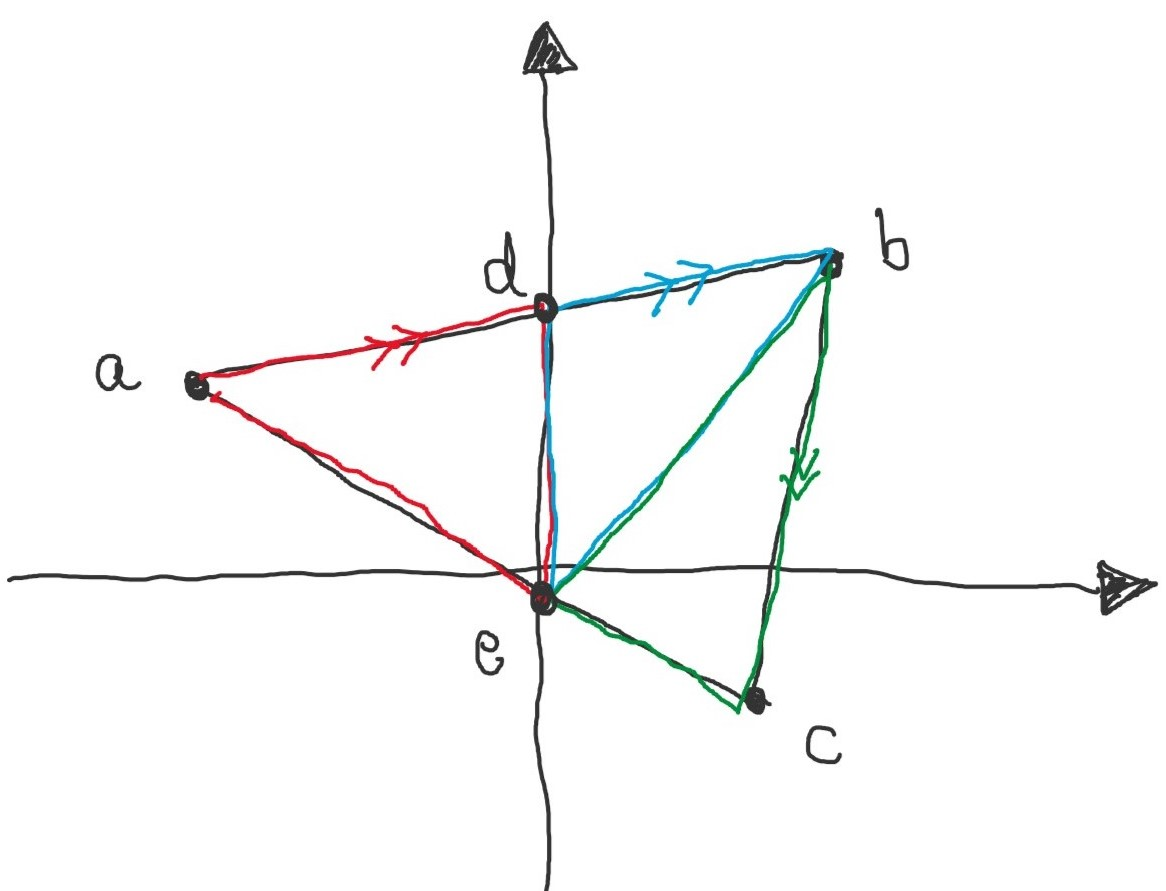
\includegraphics[height=3.5cm]{fkt_uebungen-5-abb.jpg}
	\end{center}
	Die Summe aller drei Wege ist wieder das originale Dreieck. Außerdem liegen alle \enquote{kleinen} Dreiecke nur in einer von beiden Halbebenen.
	Definiere
	\begin{equation*}
		\left.
		\begin{array}{ccccccc}
			\gamma_1 &\defeq& \sigma_{a,d} &\dot{+}& \sigma_{d,e} &\dot{+}& \sigma_{e,a} \\
			\gamma_2 &\defeq& \sigma_{d,b} &\dot{+}& \sigma_{b,e} &\dot{+}& \sigma_{e,d} \\
			\gamma_3 &\defeq& \sigma_{b,c} &\dot{+}& \sigma_{c,e} &\dot{+}& \sigma_{e,b} \\
		\end{array} 
		\right\} \follows
		\gamma = \gamma_1 \dot{+} \gamma_2 \dot{+} \gamma_3
	\end{equation*}
	wobei $\im(\gamma_1) \subseteq \quer{\CC^-}$ und $\im(\gamma_2), \im(\gamma_3) \subseteq \quer{\CC^+}$. Mit dem Hinweis gilt dann
	\begin{equation*}
		\int_{\gamma_i} f(z) \dz = 0 \quad \text{ für alle } i \in \menge{1,2,3}
	\end{equation*}
	Somit ist dann auch $\int_{\triangle(a,b,c)} f(z) \dz = 0$.
		
		
	\begin{task}
		Berechnen Sie das Integral
		\begin{equation*}
			\int_{-\infty}^\infty \frac{1}{1 + x^2} \dx
		\end{equation*}
		auf folgende Weise: Sei $R > 2$ und $\gamma_R$ der nebenstehende geschlossene Weg. Ermitteln Sie $\int_{\gamma_R} \frac{1}{1 + x^2} \dx$ mithilfe der Cauchyschen Integralformel und benutze $1 + z^2 = (z+\i) (z - \i)$. Dann Grenzübergang $R \to \infty$. 
		
		Hier darf folgende Variante des Zentrierungslemmas ohne Beweis verwendet werden: Ist $\abb{f}{\menge{z \in \CC : \Im(z) > -\frac{1}{2}} \setminus \menge{\i}}{\CC}$ holomorph, so gilt $\int_{\gamma_R} f(z) \dz = \int_{\abs{z-\i} = 1} f(z) \dz$.
		
		Berechnen Sie obiges Integral zur Probe auch mithilfe einer Stammfunktion von $x \mapsto \frac{1}{1 + x^2}$.
	\end{task}

	Parametrisiere den Weg $\gamma_R = \gamma_R^1 \dot{+} \gamma_R^2$ wie folgt: $\gamma_R^1 \defeq \id_{[-R,R]}$ und $\gamma_R^2(t) \defeq R*e^{\i t}$ für $t \in [0,\pi]$. Dann gilt 
	\begin{equation*}
		\abs{\int_{\gamma_R^2} \frac{1}{1+x^2} \dx} \le \pi R * \sup\menge{\abs{\frac{1}{1+x^2}} : \abs{x}=R, \Im(x) \ge 0} \le \frac{\pi R}{1 + R^2} \to 0 \tag{$R \to \infty$}
	\end{equation*}
	Mit der Cauchyschen Integralformel (CIF) erhält man dann
	\begin{align*}
		\lim_{R \to \infty} \int_{-R}^R \frac{1}{1 + x^2} \dx 
		&= \lim_{R \to \infty} \int_{\gamma_R^1} \frac{1}{1 + z^2} \dz \\
		&= \lim_{R \to \infty} \int_{\gamma_R} \frac{1}{1 + z^2} \dz \\
		&= \lim_{R \to \infty} \int_{\abs{z - \i} = 1} \frac{1}{(z- \i)(z + \i)} \dz \\
		&= \lim_{R \to \infty} 2\pi \i * \frac{1}{2\i}  \tag{CIF} \\
		&= \pi
	\end{align*}
	Zur Probe: Für $f(x) = \frac{1}{1 + x^2}$ ist eine Stammfunktion gegeben durch $F(x) = \arctan(x)$. Dann ist
	\begin{equation*}
		\int_{-\infty}^\infty f(x) \dx = \lim_{R \to \infty} \int_{-R}^R \frac{1}{1 + x^2} \dx = \lim_{R \to \infty} \brackets{\arctan(R) - \arctan(-R)} = \frac{\pi}{2} - \brackets{-\frac{\pi}{2}} = \pi
	\end{equation*}

	
	\begin{task}
		Sei $\abb{\gamma}{[0,1]}{\CC}$ ein geschlossener Weg. Zeigen Sie:
		\begin{equation*}
			\gamma \text{ nullhomotop} \follows \gamma \text{ nullhomolog}
		\end{equation*}		
	\end{task}

	Sei $\Omega \subseteq \CC$ offen und $\gamma$ nullhomotop in $\Omega$, d.h. homotop zu einem konstanten Weg $\abb{c}{[0,1]}{\CC}$. Dann gilt nach einer Bemerkung der Vorlesung für alle $\abb{f}{\Omega}{\CC}$ holomorph, dass $\int_\gamma f(z) \dz = \int_c f(z) \dz$. Da $c$ konstant ist, ist 
	\begin{equation*}
		\int_c f(z) \dz = \int_0^1 f(c(t)) * \underbrace{c'(t)}_{=0} \dt = 0
	\end{equation*}
	und somit also $\int_\gamma f(z) \dz = 0$ für alle holomorphen $\abb{f}{\Omega}{\CC}$. Nach Folgerung 9.4 ist dies äquivalent zur Nullhomologie von $\gamma$.
	
	
	\begin{task}
		Beweisen Sie das \textit{Schwarzsche Lemma}: Sei $\abb{f}{E}{E}$ eine holomorphe Abbildung der Einheitskreisscheibe $E$ in sich selbst mit $f(0) = 0$. Dann gilt $\abs{f'(0)} \le 1$ und $\abs{f(z)} \le \abs{z}$ für alle $z \in E$. Gibt es ein $z_0 \neq 0$ mit $\abs{f(z_0)} = \abs{z_0}$ oder gilt $\abs{f'(0)} = 1$, so ist $f$ eine Drehung mit $f(z) = e^{\i \theta} * z$ für ein $\theta \in \R$ und alle $z \in E$.
	\end{task}

	Wir definieren uns eine Funktion 
	\begin{equation*}
		\abb{g}{E}{\CC} \mit g(z) \defeq \begin{cases}
		\frac{f(z)}{z} & \text{falls } z \neq 0 \\
		f'(0)		   & \text{falls } z = 0
		\end{cases}
	\end{equation*}
	Damit ist $g$ stetig, denn
	\begin{equation*}
		g(0) = f'(0) = \lim_{z \to 0} \frac{f(z) - f(0)}{z - 0} = \lim_{z \to 0} \frac{f(z)}{z} = \lim_{\substack{z \to 0 \\ z \neq 0}} g(z)
	\end{equation*}
	Damit ist dann auch $g$ holomorph auf $E$. Für $r < 1$ gilt mit dem Maximumprinzip für $\abs{z} \le r$ 
	\begin{equation*}
		\abs{g(z)} \le \max_{\abs{z} = r} \abs{g(z)} = \frac{1}{r} * \max_{\abs{z} = r} \abs{f(z)} \le \frac{1}{r} \le 1
	\end{equation*}
	Somit ist also $\abs{g(z)} \le 1$ für alle $z \in E$, d.h. $\abs{\frac{f(z)}{z}} = \frac{\abs{f(z)}}{\abs{z}} \le 1 \follows \abs{f(z)} \le \abs{z}$ und $\abs{f'(0)} \le 1$.
	Ist $\abs{f(z_0)} = \abs{z_0}$ für ein $z_0 \neq 0$ oder $\abs{f'(0)} = 1$, so hat $\abs{g}$ im Inneren von $E$ ein lokales Maximum, was nach dem Maximumprinzip bedeutet, dass $g$ konstant ist, d.h. $g \equiv \lambda$ für ein $\lambda \in \CC$ mit $\abs{\lambda} = 1$ bzw. in Polardarstellung von $\lambda = e^{\i \theta}$ mit $\theta \in \R$ geschrieben als $f(z) = e^{\i \theta} * z$ für alle $z \in E$.
\end{exercisePage}